\chapter{Firegex}


Firegex è un firewall innovativo e multifunzionale, ideato per essere avviato con 0 configurazioni e in maniera molto rapida e semplice, che agisce principalmente a
livello applicativo di modo da permettere l'individuazione e il filtraggio del traffico in modo più intelligente e specifico per servizio.
Firegex ha diversi moduli che permettono la creazione di filtri in modo semplice, flessibile e quanto meno invasivo e impattante sulle prestazioni della macchina,
mantenendo la massima priorità sulla disponibilità e reattività del servizio stesso.
Il contesto per cui è stato pensato è quello delle competizioni CTF di tipo Attack/Defense, dove le caratteristiche precedentemente citate sono fondamentali
per semplificare l'azione difensiva in queste gare, e soprattutto dispone della flessibilità necessaria ad adattarsi ai contesti proprosti in queste competizioni.
\begin{figure}[H]
    \centering
    \begin{minipage}[b]{0.7\textwidth}
        \centering
        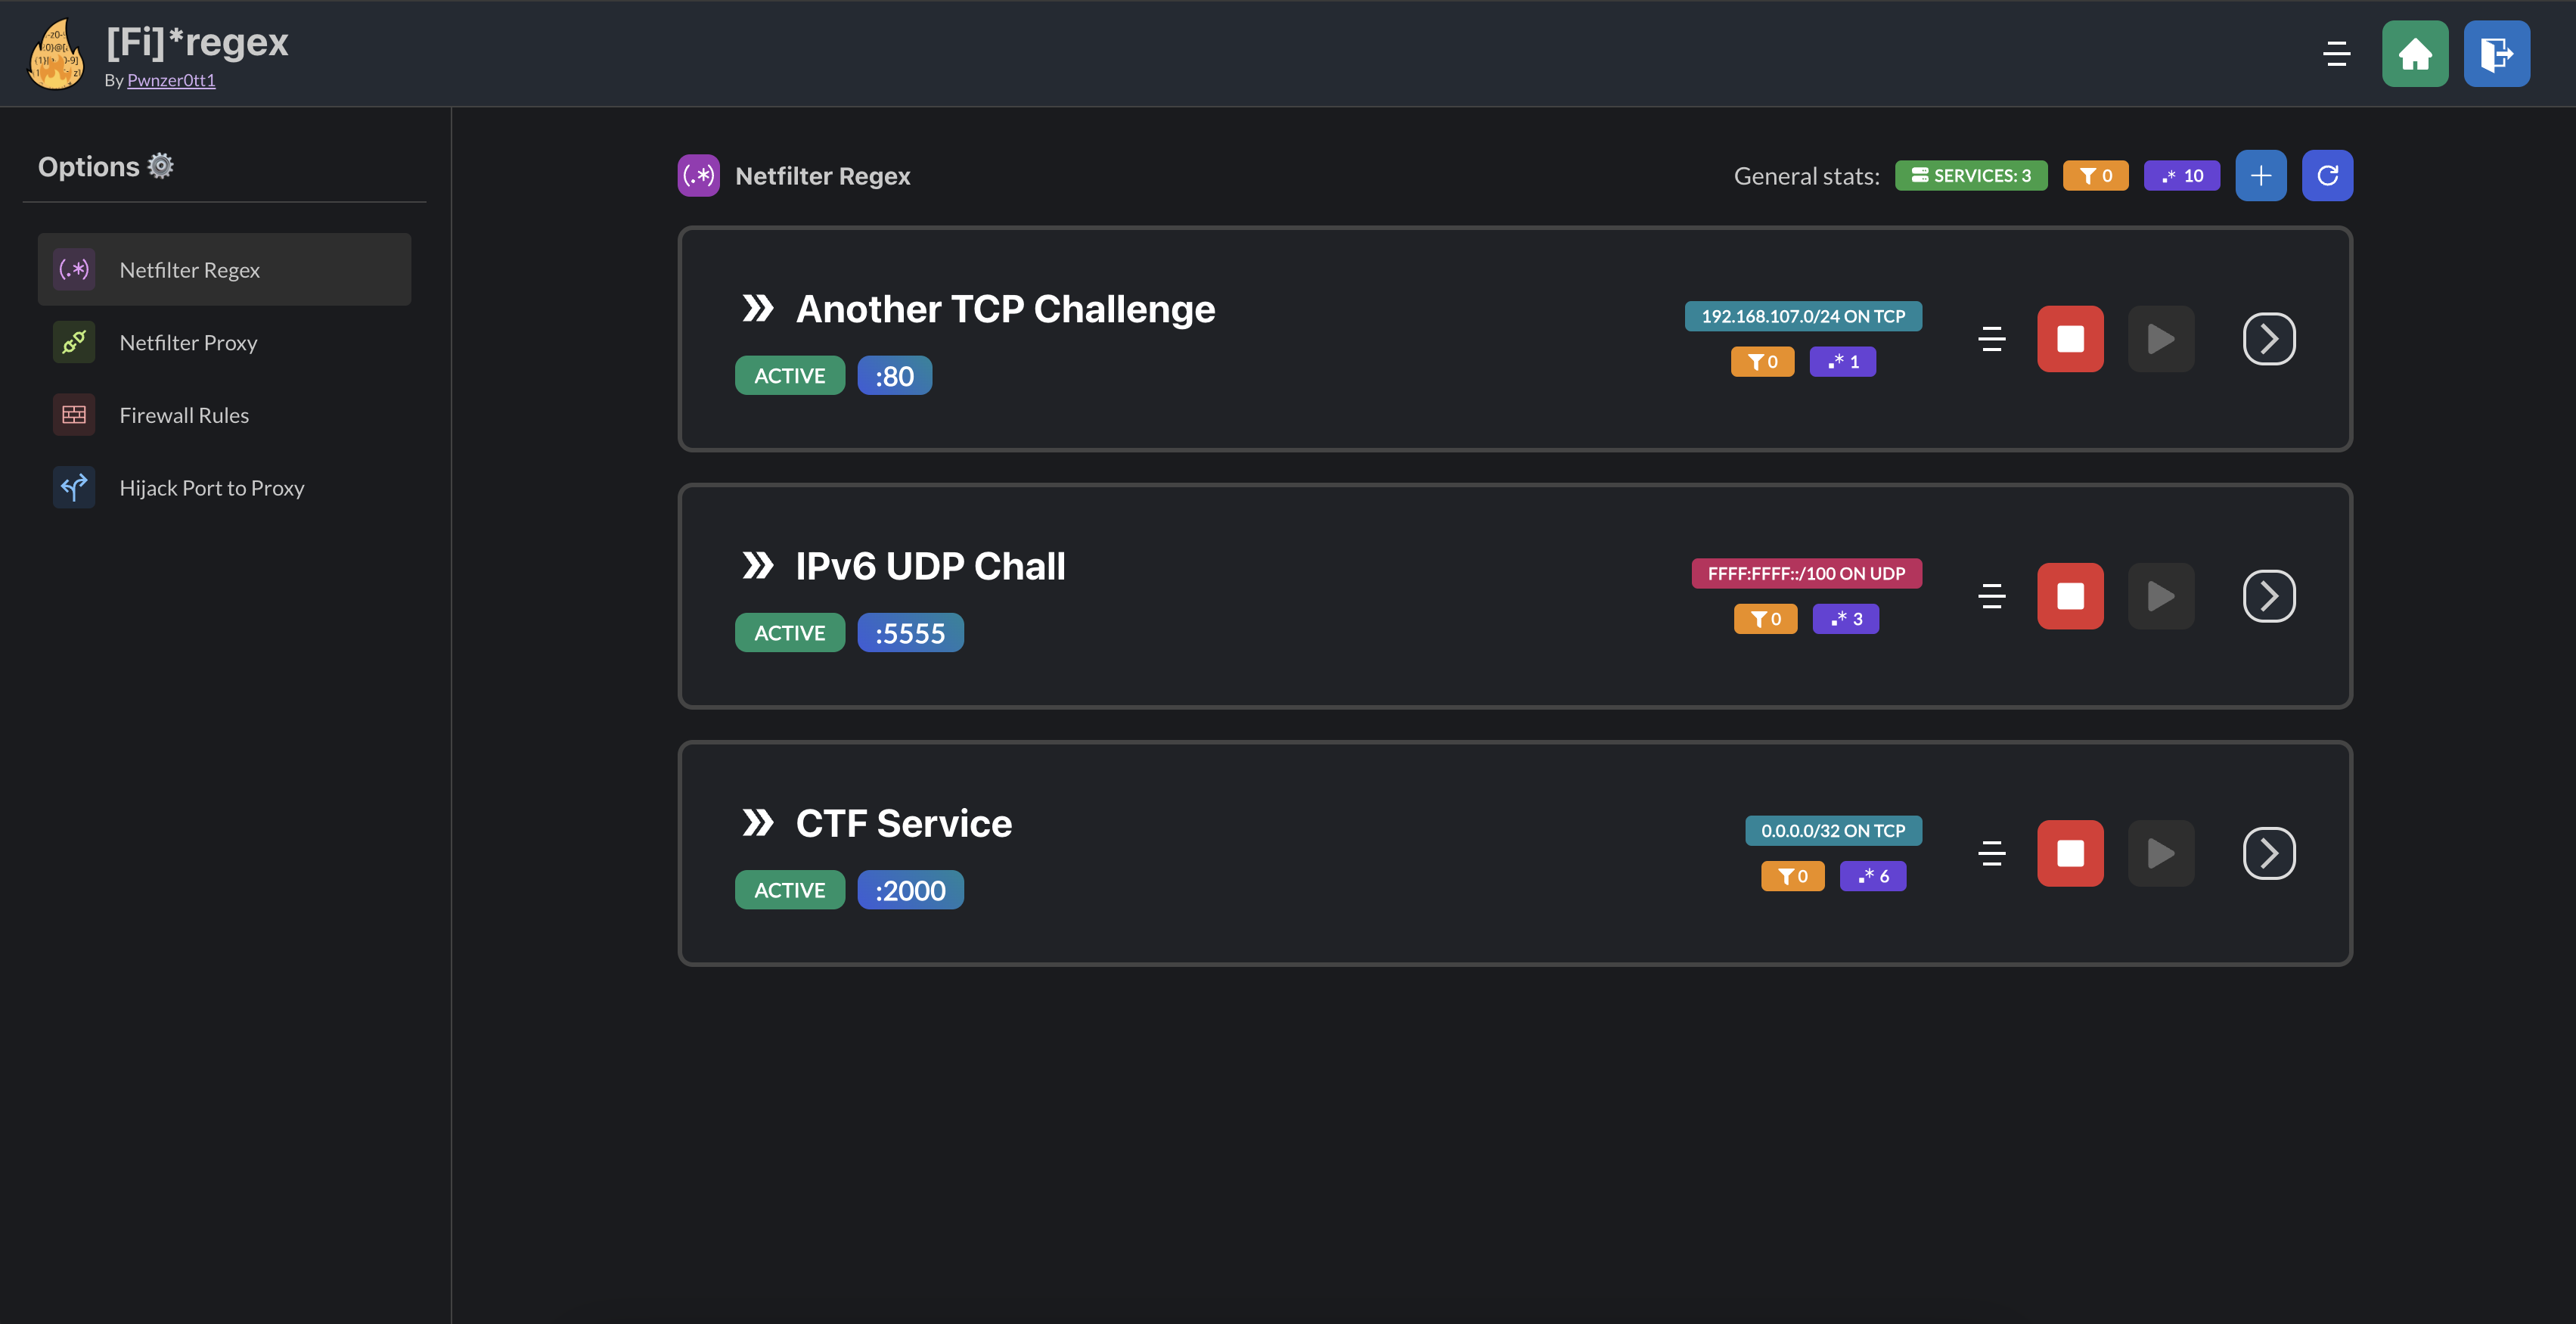
\includegraphics[width=1\textwidth]{images/chapter2/Firegex_Screenshot.png}
        \caption{Interfaccia grafica di Firegex}
        \label{fig:firegex_frontend}
    \end{minipage}
    \begin{minipage}[b]{0.7\textwidth}
        \centering
        
\includegraphics[width=0.20\textwidth]{images/chapter2/FiregexLogo.png}
        \caption{Logo di Firegex}
        \label{fig:firegex_logo}
    \end{minipage}
\end{figure}


\section{Perché nasce Firegex?}

Firegex (come precedentemente detto) nasce dal gruppo che ha affrontato la gara nazionale Cyberchallenge\footcite{\url{https://cyberchallenge.it/}}{cyberchallenge}
del 2022 al Politecnico di Bari, e nasce come un normale proxy con filtraggio tramite l'ausilio di regex, col tempo rimpiazzato con funzioni simili, ma più efficienti e sicure.\\
La necessità dello sviluppo è nata proprio dalla mancanza di un sistema di difesa che fosse immediato da usare, che non richiedesse configurazioni complesse per
essere avviato, e che permettesse in maniera molto semplice di costruire dei filtri immediatamente attivi e funzionanti.\\

Durante il suo sviluppo firegex ha acquisito ulteriori funzionalità e requisiti:

\begin{itemize}
    \item \textbf{Trasparenza totale:} La creazione di un proxy comporta una serie di cambiamenti lato gestione delle porte esposte dai servizi, avvio del proxy stesso,
    e gestione di fallback in caso di problemi legati al proxy. Queste complicanze erano solo parzialmente gestite inizialmente da firegex, ma con le nuove implementazioni
    è possibile applicare regola sul traffico senza cambiamenti di configurazione, e in maniera immediata interagendo direttamente con il kernel linux, ma nascondendo
    all'utilizzatore finale tutta la complessità gestita internamente.
    \item \textbf{Integrazione di tecnologie multiple:} Inizialmente firegex (come deducibile dal nome) aveva come principale e unico sistema di filtraggio le regex,
    applicate sui pacchetti di rete per individuare eventuali attacchi. Negli anni si è notato come questo approccio spesso potesse essere limitante, pertanto sono state
    implementate diverse tecnologie di filtraggio discusse meglio in seguito per aumentare la flessibilità sui filtri applicabili. La seguente tesi tratterà dello sviluppo
    di una nuova funzionalità particolarmente flessibile denominata \texttt{nfproxy}.
    \item \textbf{Affidabilità e disponibilità:} In ambienti dove la continuità del servizio è critica, è fondamentale che il sistema di sicurezza non diventi un
    collo di bottiglia. Firegex è stato progettato per garantire un’elevata disponibilità, offrendo soluzioni rapide per il ripristino della configurazione in
    caso di errori e per il reset immediato dei filtri applicati, erroneamente scritti.
    \item \textbf{Facilità di utilizzo:} Nelle A/D il tempo è una risorsa fondamentale necessariamente da ottimizzare per concentrare le risorse su attività legate
    all'individuazione di vulnerabilità, che rappresenta il cuore della competizione. Firegex è stato progettato per essere quanto meno dispersivo possibile,
    con configurazioni semplici, un'interfaccia intuitiva, e per gestire autonomamente tutte le problematiche legate alla gestione dei filtri, alla configurazione
    del kernel e all'inserimento di regole di rete.
\end{itemize}

\section{Confronto con altre soluzioni}

Firegex si distingue rispetto ad altre soluzioni open-source presenti, come
\texttt{CTF proxy}\footcite{\url{https://github.com/ByteLeMani/ctf_proxy}}{ctf_proxy},
\texttt{Nginx}\footcite{\url{https://nginx.org/}}{nginx}, \texttt{Suricata}\footcite{\url{https://suricata.io/}}{suricata}
o \texttt{Fortinet}\footcite{\url{https://www.fortinet.com/}}{fortinet} per diversi motivi:\\

\renewcommand{\arraystretch}{2}
\begin{table}[H]
    \centering
    \setlength{\tabcolsep}{12pt}
    \begin{tabular}{|c|c|c|c|c|}
        \hline
        \begin{tabular}[c]{@{}c@{}} \textbf{Firewall} \end{tabular} & 
        \begin{tabular}[c]{@{}c@{}} \textbf{0 Config Run}  \end{tabular} & 
        \begin{tabular}[c]{@{}c@{}} \textbf{Easy use} \end{tabular} & 
        \begin{tabular}[c]{@{}c@{}} \textbf{Easy Filter Add} \end{tabular} & 
        \begin{tabular}[c]{@{}c@{}} \textbf{Flexible} \end{tabular} \\
        \hline
        \texttt{Firegex} & 
        \begin{tabular}[c]{@{}c@{}} \color{Green}\faIcon[solid]{check-circle} \end{tabular} & 
        \begin{tabular}[c]{@{}c@{}} \color{Green}\faIcon[solid]{check-circle} \end{tabular} & 
        \begin{tabular}[c]{@{}c@{}} \color{Green}\faIcon[solid]{check-circle} \end{tabular} & 
        \begin{tabular}[c]{@{}c@{}} \color{Green}\faIcon[solid]{check-circle} \end{tabular} \\
        \hline
        \texttt{Nginx} & 
        \begin{tabular}[c]{@{}c@{}} \color{Orange}\faIcon[solid]{exclamation-circle} \end{tabular} & 
        \begin{tabular}[c]{@{}c@{}} \color{Orange}\faIcon[solid]{exclamation-circle} \end{tabular} & 
        \begin{tabular}[c]{@{}c@{}} \color{Orange}\faIcon[solid]{exclamation-circle} \end{tabular} & 
        \begin{tabular}[c]{@{}c@{}} \color{Orange}\faIcon[solid]{exclamation-circle} \end{tabular} \\
        \hline
        \texttt{CTF proxy} & 
        \begin{tabular}[c]{@{}c@{}} \color{Red}\faIcon[solid]{times-circle} \end{tabular} & 
        \begin{tabular}[c]{@{}c@{}} \color{Orange}\faIcon[solid]{exclamation-circle} \end{tabular} & 
        \begin{tabular}[c]{@{}c@{}} \color{Orange}\faIcon[solid]{exclamation-circle} \end{tabular} & 
        \begin{tabular}[c]{@{}c@{}} \color{Green}\faIcon[solid]{check-circle} \end{tabular} \\
        \hline
        \texttt{Fortinet} & 
        \begin{tabular}[c]{@{}c@{}} \color{Red}\faIcon[solid]{times-circle} \end{tabular} & 
        \begin{tabular}[c]{@{}c@{}} \color{Red}\faIcon[solid]{times-circle} \end{tabular} & 
        \begin{tabular}[c]{@{}c@{}} \color{Orange}\faIcon[solid]{exclamation-circle} \end{tabular} & 
        \begin{tabular}[c]{@{}c@{}} \color{Orange}\faIcon[solid]{exclamation-circle} \end{tabular} \\ 
        \hline
        \texttt{Suricata} & 
        \begin{tabular}[c]{@{}c@{}} \color{Red}\faIcon[solid]{times-circle} \end{tabular} & 
        \begin{tabular}[c]{@{}c@{}} \color{Orange}\faIcon[solid]{exclamation-circle} \end{tabular} & 
        \begin{tabular}[c]{@{}c@{}} \color{Orange}\faIcon[solid]{exclamation-circle} \end{tabular} & 
        \begin{tabular}[c]{@{}c@{}} \color{Orange}\faIcon[solid]{exclamation-circle} \end{tabular} \\
        \hline
    \end{tabular}
    \caption{Confronto tra le soluzioni per il firewall}
    \label{tab:firewall_compare}
\end{table}
\renewcommand{\arraystretch}{1}

\begin{itemize}
    \setlength{\itemsep}{5pt}
    \setlength{\parskip}{5pt}
    \item \texttt{Nginx} è una soluzione molto flessibile e affidabile, ma richiede configurazioni complesse e non permette di applicare filtri in maniera
    immediata e trasparente, ha necessità di cambiare porte e non supporta nativamente filtri più avanzati come quello trattato in questa tesi. 
    Non ha una interfaccia grafica per la gestione delle regole.
    \item \texttt{CTF proxy} è una soluzione molto flessibile e affidabile, ma richiede la creazione di configurazioni e allo stesso modo necessita di cambiare porte
    ai servizi originali, inoltre a suo supporto non esiste un'interfaccia semplice da usare.
    \item \texttt{Fortinet} è una soluzione molto affidabile e flessibile, ben riconosciuta nel settore, ma richiede configurazioni complesse
    è molto lento da configurare, e la configurazione stessa può causare diversi problemi, essendo molto invasiva nel sistema, e molto lenta.
    Il suo utilizzo è molto complesso e poco pratico per le competizioni CTF. Filtri più complessi necessintano la scrittura di appositi plugin poco rapidi da sviluppare.
    Rappresenta una delle principali soluzioni fuori dal contesto delle competizioni CTF.
    \item \texttt{Suricata} è una soluzione molto affidabile che offre un grado intermedio di flessibilità, non ha un'interfaccia semplice per il suo utilizzo,
    richiede conffigurazioni per essere avviato.
\end{itemize}

\section{Architettura}

Firegex avendo un interfaccia web è composto da un frontend scritto in \texttt{react}\footcite{\url{https://react.dev/}}{react}
e un backend scritto in \texttt{fastapi}\footcite{\url{https://fastapi.tiangolo.com/}}{fastapi}.
Il backend utilizza inoltre dei moduli scritti in C++ per le funzionalità più critiche, come il filtraggio diretto a livello kernel e l'elaborazione in tempo reale delle espressioni regolari.
Inoltre per funzionare, firegex fa intenso utilizzo delle funzionalità di \texttt{nftables}\footcite{\url{https://netfilter.org/projects/nftables/}}{nftables}, e di
\texttt{netfilter\_queue}\footcite{\url{https://netfilter.org/projects/libnetfilter_queue/}}{netfilter_queue} (brevemente \texttt{nfqueue}).
Firegex è basato su \texttt{docker}\footcite{\url{https://www.docker.com/}}{docker} che ne permette un avvio con 0 configurazione e immediato: \texttt{docker} è usualmente lo
strumento principale per l'avvio di servizi in competizioni CTF, pertanto nella maggior parte dei casi è già presente e configurato correttamente.

\begin{figure}[H]
    \centering
    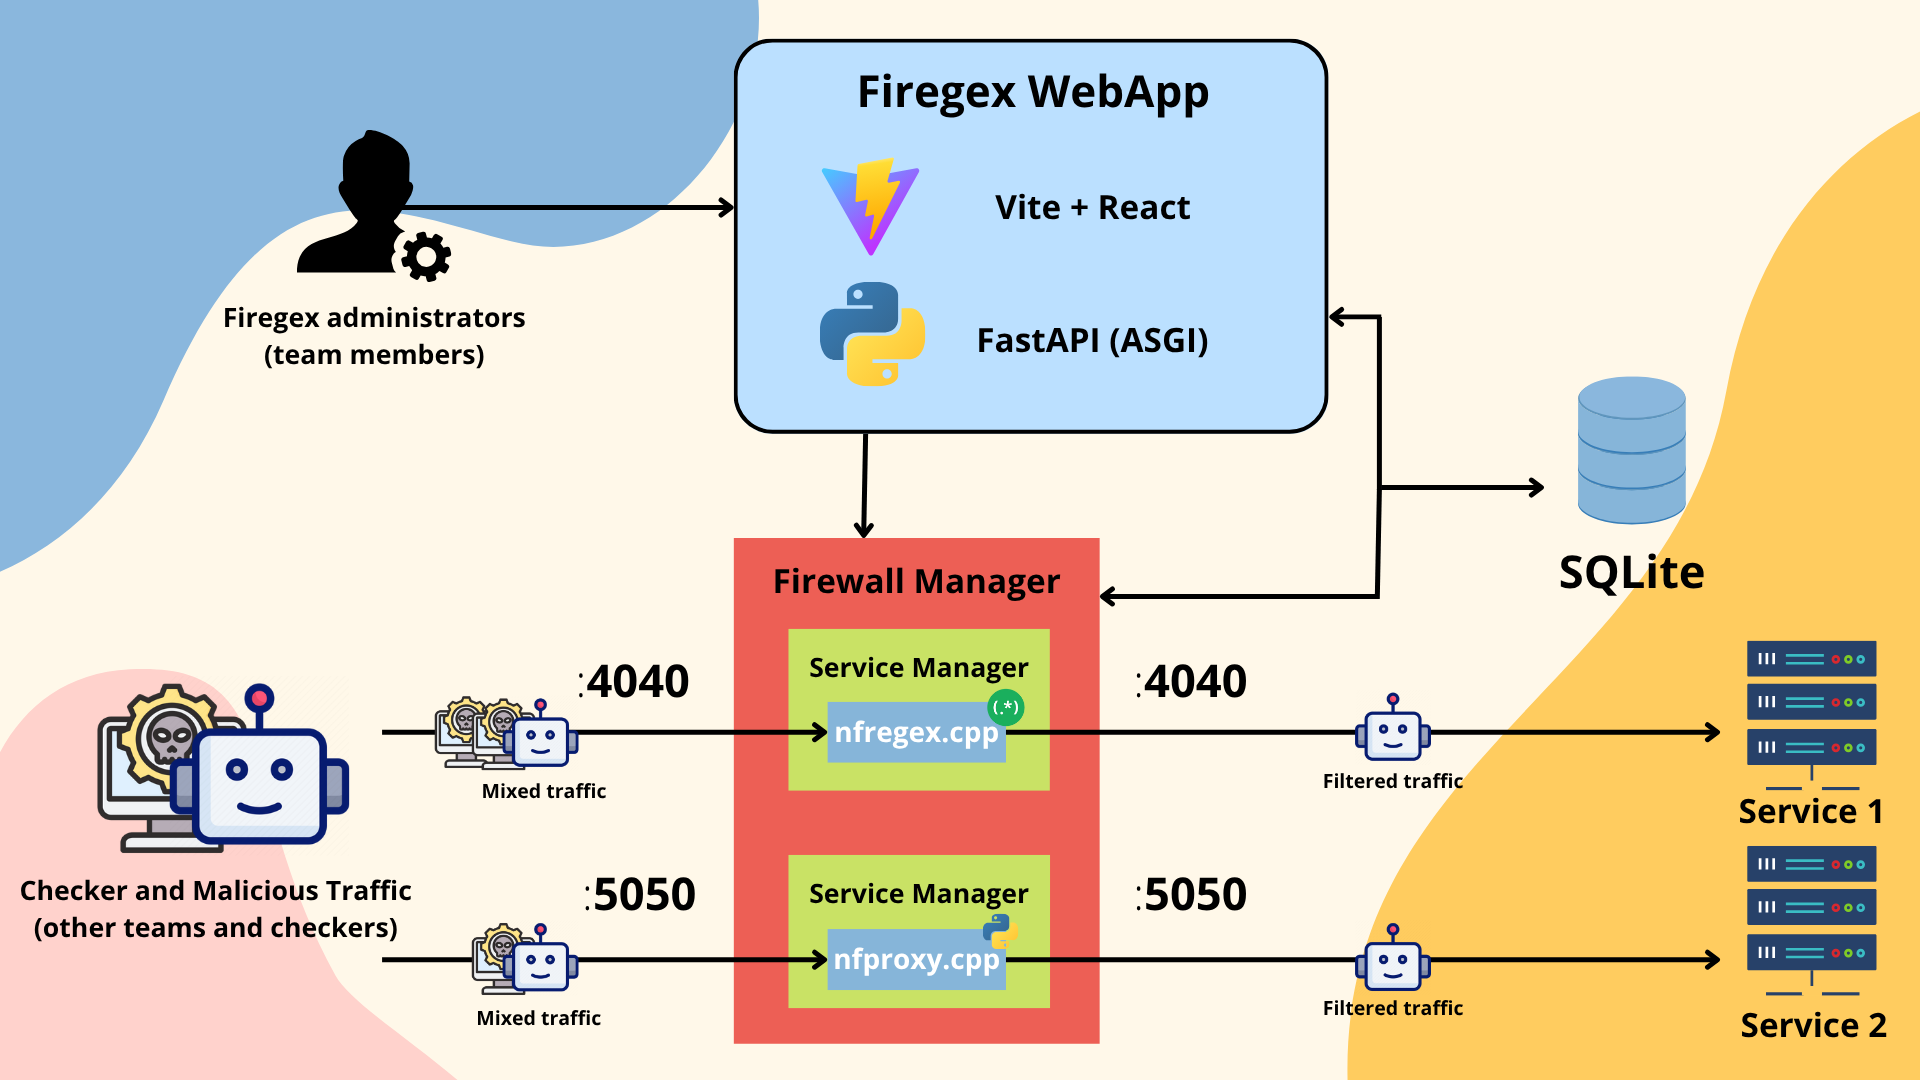
\includegraphics[width=0.58\textwidth]{images/chapter2/FiregexInternals.png}
    \caption{Schema generale dell'architettura di Firegex}
    \label{fig:firegex_arch}
\end{figure}

\subsection{Frontend e Backend}
\begin{itemize}
    \item \textbf{Frontend (React):} L'interfaccia utente è sviluppata in React, offrendo una piattaforma interattiva e intuitiva per la configurazione, il monitoraggio
    e la gestione delle regole di sicurezza. L'interfaccia è parte fondamentale di Firegex, poichè consente di soddisfare uno dei punti chiave del progetto: la semplicità di utilizzo.
    \item \textbf{Backend (FastAPI + C++):} Il backend è realizzato utilizzando FastAPI, un framework moderno e ad alte prestazioni per la creazione di API, integrato
    con moduli critici scritti in C++. Questa combinazione consente di gestire le richieste in maniera estremamente veloce e affidabile, garantendo al contempo la possibilità
    di eseguire operazioni critiche a velocità ottimali per essere integrate nei moduli per la gestione della rete. Il backend tuttavia svolge anche un ruolo attivo nell'applicazione
    delle regole di rete tramite il wrap python ufficiale di \texttt{libnftables}\footcite{\url{https://git.netfilter.org/nftables/tree/py}}{nftables_python}.
\end{itemize}

\subsection{Moduli C++}
Il cuore delle funzionalità critiche di Firegex è implementato in C++. Questi moduli sono responsabili del filtraggio diretto a livello kernel per i moduli \texttt{nfregex} e \texttt{nfproxy},
e fanno utilizzo di librerie ad altre prestazioni ed adatte all'utilizzo in networking come
\texttt{libtins}\footcite{\url{https://libtins.github.io/}}{libtins}, \texttt{libmnl}\footcite{\url{https://netfilter.org/projects/libmnl/}}{libmnl},
\texttt{vectorscan}\footcite{\url{https://vectorcamp.gr/project/vectorscan/}}{vectorscan} (specificatamente per \texttt{nfregex}),
e delle C API di \texttt{python}\footcite{\url{https://docs.python.org/3/c-api/}}{python_c_api} (specificatamente per \texttt{nfproxy}).

\begin{itemize}
    \item \textbf{Prestazioni elevate:} Grazie all'efficienza del linguaggio C++ e alla sua integrazione diretta con le chiamate di sistema, il filtraggio e
    l'analisi del traffico avvengono con tempi di latenza estremamente ridotti.
    \item \textbf{Parallelizzazione:} I filtri che richiedono elaborazione userspace facendo uso di nfqueue, sono sempre disponibili per l'elaborazione multi-thread,
    garantendo una gestione ottimale del traffico in situazioni di carico elevato.
    \item \textbf{Integrazione con librerie di rete:} L'utilizzo di librerie specializzate come libtins e libmnl consente di implementare funzionalità avanzate
    con avendo grande affidabilità sulle operazioni di rete e prestazioni nell'elaborazione dei pacchetti.
\end{itemize}

\subsection{Netfilter nftables}
nftables rappresenta il framework moderno per il filtraggio dei pacchetti e la gestione del traffico nelle distribuzioni Linux. In Firegex, nftables viene utilizzato per:
\begin{itemize}
    \item \textbf{Applicare regole di sicurezza:} Le regole di firewall vengono implementate tramite nftables, garantendo un controllo granulare sul traffico di rete.
    \item \textbf{Reindirizzamento del traffico:} La funzionalità di \texttt{porthijack} si basa su regole di nftables per deviare il traffico da una porta
    a un’altra, consentendo l’implementazione di proxy interni o la segmentazione del traffico sospetto.
    \item \textbf{Integrazione con nfqueue:} nftables lavora in sinergia con il modulo nfqueue per intercettare i pacchetti e inoltrarli allo spazio
    utente per ulteriori analisi.
\end{itemize}

\subsection{Netfilter Queue Module}
Il modulo Netfilter Queue (nfqueue) gioca un ruolo fondamentale nell'architettura di Firegex, consentendo l'intercettazione dei pacchetti direttamente
a livello kernel e il loro inoltro allo spazio utente. Le sue principali caratteristiche includono:
\begin{itemize}
    \item \textbf{Intercettazione diretta:} nfqueue permette di catturare internamente il traffico di rete: questo rende accessibile allo sviluppatore accesso dal layer di network in su
    permettendo anche l'analisi e la modifica degli header dei pacchetti normalmente non accessibili tramite un proxy. Inoltre intercettare i pacchetti in questo modo rende l'operazione di filtraggio completamente
    invisibile per l'applicativo, che non bisognerà manomettere in alcun modo.
    \item \textbf{Elaborazione in spazio utente:} Una volta intercettati, i pacchetti vengono inoltrati allo spazio utente dove possono essere analizzati e
    processati da moduli come \texttt{nfregex} e \texttt{nfproxy}, consentendo l'utilizzo di logiche di filtraggio avanzate ma comunque evitando di portare codice potenzialmente pericoloso
    lato kernel che potrebbe compromettere la stabilità del sistema.
\end{itemize}

\section{Funzionalità}

All'interno di Firegex sono presenti attualmente 4 moduli principali, ognuno con delle funzionalità specifiche che permettono di applicare filtri in maniera
differente. I moduli sono \texttt{nfregex}, \texttt{firewall}, \texttt{porthijack} e \texttt{nfproxy}. All'interno di questi moduli firegex possiede una documentazione
interna alla piattaforma stessa che permette di comprendere come utilizzare le funzionalità offerte, e come configurare i filtri in maniera corretta.\\
Come citato precedentemente firegex è avviabile tramite un one-command: '\texttt{sh <(curl -sLf https://pwnzer0tt1.it/firegex.sh)}'

\subsection{nfregex}
Il modulo \texttt{nfregex} rappresenta la funzionalità (pensata originariamente come l'unica e principale) basata su filtri scritti con espressioni regolari. Utilizzando nfqueue in combinazione con
\texttt{nftables}, questo modulo intercetta le richieste di rete direttamente a livello kernel. La funzionalità permette l'utilizzo di regex
\texttt{PCRE2}\footcite{\url{https://www.pcre.org/}}{pcre_website} compliant tramite l'utilizzo di \texttt{vectorscan}\footcite{\url{https://vectorcamp.gr/project/vectorscan/}}{vectorscan}
(fork di \texttt{hyperscan}\footcite{\url{http://hyperscan.io/}}{hyperscan} compatibile con arm64) per garantire prestazioni elevate
e una valutazione accurata delle regole. La funzionalità supporta IPv4, IPv6 e protocolli di livello superiore come TCP, UDP.
Per i pacchetti TCP, la regex viene applicata all'intero flusso ricostruito e ordinato tramite le \texttt{stream regex} offerte da vectorscan.

\subsection{firewall}
La funzionalità \texttt{firewall} di Firegex si propone di offrire un controllo completo sul traffico di rete, simile a quanto si ottiene con strumenti
tradizionali come \texttt{ufw} o \texttt{iptables}. Ha funzionalità di base ed è utile per evitare l'utilizzo di ulteriori tool di filtering che potrebbero andare in conflitto con firegex.

\subsection{porthijack}
Il modulo \texttt{porthijack} introduce la capacità di reindirizzare il traffico destinato a una determinata porta verso un’altra. Questa funzionalità è particolarmente utile in scenari dove
si ha il bisogno di costruire un proxy personalizzato, ma si vuole evitare la riconfigurazione del servizio di base.
Port hijacking infatti consente di impostare un redirect del traffico dall'interfaccia su cui il servizio viene esposto nella rete di gare, facendolo passare per un proxy
in localhost, che poi tramite la stessa interfaccia di loopback inoltrerà il traffico al servizio originale.

\subsection{nfproxy}
\texttt{nfproxy} è il modulo trattato in questa tesi che sfrutta il meccanismo nfqueue per simulare il comportamento di un proxy sviluppato in Python. Le caratteristiche
principali di questa funzionalità sono:
\begin{itemize}
    \item \textbf{Sviluppo in Python:} Permette agli sviluppatori di scrivere e integrare filtri personalizzati in linguaggio Python, offrendo un ambiente flessibile
    per l'analisi del traffico.
    \item \textbf{Parsing avanzato dei protocolli:} Include handler predefiniti per il parsing di protocolli come HTTP, facilitando la realizzazione di filtri sofisticati.
    \item \textbf{Test e validazione:} I filtri possono essere testati in anticipo tramite il comando \texttt{fgex}, rendendo possibile la prova del filtro prima dell'effettiva applicazione.
\end{itemize}

Il seguente modulo è stato introdotto in vista di scenari complessi dove gli elementi da individuare per un corretto filtraggio non sono facilmente
individuabili tramite regex, e dove è necessario un controllo più granulare sul traffico.\\
Ad esempio se l'attacco avvenisse nei cookie JWT sarebbe necessario eseguire il decoding del token per individuare l'attacco, cosa non possibile con nfregex.\\

Nei prossimi capitoli verrà trattato in dettaglio lo sviluppo di \texttt{nfproxy}, le sue funzionalità, le sue caratteristiche e le sue prestazioni.

\begin{figure}[H]
    \centering
    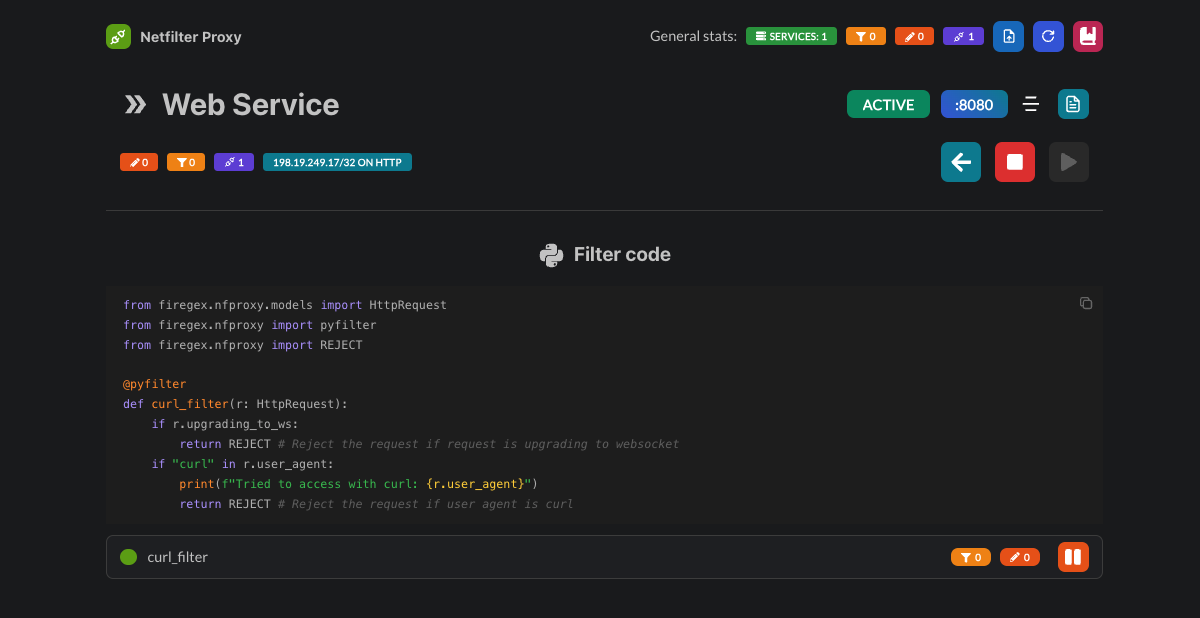
\includegraphics[width=0.8\textwidth]{images/chapter2/NFProxyInterface.png}
    \caption{Interfaccia di dettaglio del servizio nel modulo nfproxy}
    \label{fig:nfproxy_interface}
\end{figure}

